\documentclass[twoside]{book}

% Packages required by doxygen
\usepackage{fixltx2e}
\usepackage{calc}
\usepackage{doxygen}
\usepackage[export]{adjustbox} % also loads graphicx
\usepackage{graphicx}
\usepackage[utf8]{inputenc}
\usepackage{makeidx}
\usepackage{multicol}
\usepackage{multirow}
\PassOptionsToPackage{warn}{textcomp}
\usepackage{textcomp}
\usepackage[nointegrals]{wasysym}
\usepackage[table]{xcolor}

% Font selection
\usepackage[T1]{fontenc}
\usepackage[scaled=.90]{helvet}
\usepackage{courier}
\usepackage{amssymb}
\usepackage{sectsty}
\renewcommand{\familydefault}{\sfdefault}
\allsectionsfont{%
  \fontseries{bc}\selectfont%
  \color{darkgray}%
}
\renewcommand{\DoxyLabelFont}{%
  \fontseries{bc}\selectfont%
  \color{darkgray}%
}
\newcommand{\+}{\discretionary{\mbox{\scriptsize$\hookleftarrow$}}{}{}}

% Page & text layout
\usepackage{geometry}
\geometry{%
  a4paper,%
  top=2.5cm,%
  bottom=2.5cm,%
  left=2.5cm,%
  right=2.5cm%
}
\tolerance=750
\hfuzz=15pt
\hbadness=750
\setlength{\emergencystretch}{15pt}
\setlength{\parindent}{0cm}
\setlength{\parskip}{3ex plus 2ex minus 2ex}
\makeatletter
\renewcommand{\paragraph}{%
  \@startsection{paragraph}{4}{0ex}{-1.0ex}{1.0ex}{%
    \normalfont\normalsize\bfseries\SS@parafont%
  }%
}
\renewcommand{\subparagraph}{%
  \@startsection{subparagraph}{5}{0ex}{-1.0ex}{1.0ex}{%
    \normalfont\normalsize\bfseries\SS@subparafont%
  }%
}
\makeatother

% Headers & footers
\usepackage{fancyhdr}
\pagestyle{fancyplain}
\fancyhead[LE]{\fancyplain{}{\bfseries\thepage}}
\fancyhead[CE]{\fancyplain{}{}}
\fancyhead[RE]{\fancyplain{}{\bfseries\leftmark}}
\fancyhead[LO]{\fancyplain{}{\bfseries\rightmark}}
\fancyhead[CO]{\fancyplain{}{}}
\fancyhead[RO]{\fancyplain{}{\bfseries\thepage}}
\fancyfoot[LE]{\fancyplain{}{}}
\fancyfoot[CE]{\fancyplain{}{}}
\fancyfoot[RE]{\fancyplain{}{\bfseries\scriptsize Generated by Doxygen }}
\fancyfoot[LO]{\fancyplain{}{\bfseries\scriptsize Generated by Doxygen }}
\fancyfoot[CO]{\fancyplain{}{}}
\fancyfoot[RO]{\fancyplain{}{}}
\renewcommand{\footrulewidth}{0.4pt}
\renewcommand{\chaptermark}[1]{%
  \markboth{#1}{}%
}
\renewcommand{\sectionmark}[1]{%
  \markright{\thesection\ #1}%
}

% Indices & bibliography
\usepackage{natbib}
\usepackage[titles]{tocloft}
\setcounter{tocdepth}{3}
\setcounter{secnumdepth}{5}
\makeindex

% Hyperlinks (required, but should be loaded last)
\usepackage{ifpdf}
\ifpdf
  \usepackage[pdftex,pagebackref=true]{hyperref}
\else
  \usepackage[ps2pdf,pagebackref=true]{hyperref}
\fi
\hypersetup{%
  colorlinks=true,%
  linkcolor=blue,%
  citecolor=blue,%
  unicode%
}

% Custom commands
\newcommand{\clearemptydoublepage}{%
  \newpage{\pagestyle{empty}\cleardoublepage}%
}

\usepackage{caption}
\captionsetup{labelsep=space,justification=centering,font={bf},singlelinecheck=off,skip=4pt,position=top}

%===== C O N T E N T S =====

\begin{document}

% Titlepage & ToC
\hypersetup{pageanchor=false,
             bookmarksnumbered=true,
             pdfencoding=unicode
            }
\pagenumbering{alph}
\begin{titlepage}
\vspace*{7cm}
\begin{center}%
{\Large Digiteco\+Power Library \\[1ex]\large 1 }\\
\vspace*{1cm}
{\large Generated by Doxygen 1.8.13}\\
\end{center}
\end{titlepage}
\clearemptydoublepage
\pagenumbering{roman}
\tableofcontents
\clearemptydoublepage
\pagenumbering{arabic}
\hypersetup{pageanchor=true}

%--- Begin generated contents ---
\chapter{Namespace Index}
\section{Namespace List}
Here is a list of all documented namespaces with brief descriptions\+:\begin{DoxyCompactList}
\item\contentsline{section}{\hyperlink{namespaceDigitecoPower}{Digiteco\+Power} \\*\hyperlink{namespaceDigitecoPower}{Digiteco\+Power} namespace }{\pageref{namespaceDigitecoPower}}{}
\end{DoxyCompactList}

\chapter{File Index}
\section{File List}
Here is a list of all documented files with brief descriptions\+:\begin{DoxyCompactList}
\item\contentsline{section}{sketchbook/libraries/\+Digiteco\+Power/\hyperlink{digiteco__power_8cpp}{digiteco\+\_\+power.\+cpp} }{\pageref{digiteco__power_8cpp}}{}
\item\contentsline{section}{sketchbook/libraries/\+Digiteco\+Power/\hyperlink{digiteco__power_8h}{digiteco\+\_\+power.\+h} }{\pageref{digiteco__power_8h}}{}
\item\contentsline{section}{sketchbook/libraries/\+H\+Y\+T2\+X1/\hyperlink{hyt2x1_8cpp}{hyt2x1.\+cpp} }{\pageref{hyt2x1_8cpp}}{}
\item\contentsline{section}{sketchbook/libraries/\+H\+Y\+T2\+X1/\hyperlink{hyt2x1_8h}{hyt2x1.\+h} }{\pageref{hyt2x1_8h}}{}
\item\contentsline{section}{sketchbook/libraries/\+N\+T\+P/\hyperlink{ntp_8cpp}{ntp.\+cpp} }{\pageref{ntp_8cpp}}{}
\item\contentsline{section}{sketchbook/libraries/\+N\+T\+P/\hyperlink{ntp_8h}{ntp.\+h} }{\pageref{ntp_8h}}{}
\item\contentsline{section}{sketchbook/libraries/\+P\+C\+F8563/\hyperlink{pcf8563_8cpp}{pcf8563.\+cpp} }{\pageref{pcf8563_8cpp}}{}
\item\contentsline{section}{sketchbook/libraries/\+P\+C\+F8563/\hyperlink{pcf8563_8h}{pcf8563.\+h} }{\pageref{pcf8563_8h}}{}
\item\contentsline{section}{sketchbook/libraries/\+Rmap/\hyperlink{debug_8cpp}{debug.\+cpp} }{\pageref{debug_8cpp}}{}
\item\contentsline{section}{sketchbook/libraries/\+Rmap/\hyperlink{debug_8h}{debug.\+h} }{\pageref{debug_8h}}{}
\item\contentsline{section}{sketchbook/libraries/\+Rmap/\hyperlink{eeprom__utility_8h}{eeprom\+\_\+utility.\+h} }{\pageref{eeprom__utility_8h}}{}
\item\contentsline{section}{sketchbook/libraries/\+Rmap/\hyperlink{i2c__utility_8cpp}{i2c\+\_\+utility.\+cpp} }{\pageref{i2c__utility_8cpp}}{}
\item\contentsline{section}{sketchbook/libraries/\+Rmap/\hyperlink{i2c__utility_8h}{i2c\+\_\+utility.\+h} }{\pageref{i2c__utility_8h}}{}
\item\contentsline{section}{sketchbook/libraries/\+Rmap/\hyperlink{registers-rain_8h}{registers-\/rain.\+h} }{\pageref{registers-rain_8h}}{}
\item\contentsline{section}{sketchbook/libraries/\+Rmap/\hyperlink{registers-th_8h}{registers-\/th.\+h} }{\pageref{registers-th_8h}}{}
\item\contentsline{section}{sketchbook/libraries/\+Rmap/\hyperlink{registers_8h}{registers.\+h} }{\pageref{registers_8h}}{}
\item\contentsline{section}{sketchbook/libraries/\+Rmap/\hyperlink{rmap__utility_8cpp}{rmap\+\_\+utility.\+cpp} }{\pageref{rmap__utility_8cpp}}{}
\item\contentsline{section}{sketchbook/libraries/\+Rmap/\hyperlink{rmap__utility_8h}{rmap\+\_\+utility.\+h} }{\pageref{rmap__utility_8h}}{}
\item\contentsline{section}{sketchbook/libraries/\+Rmap/\hyperlink{sdcard__utility_8cpp}{sdcard\+\_\+utility.\+cpp} }{\pageref{sdcard__utility_8cpp}}{}
\item\contentsline{section}{sketchbook/libraries/\+Rmap/\hyperlink{sdcard__utility_8h}{sdcard\+\_\+utility.\+h} }{\pageref{sdcard__utility_8h}}{}
\item\contentsline{section}{sketchbook/libraries/\+Rmap/\hyperlink{stima__module_8h}{stima\+\_\+module.\+h} }{\pageref{stima__module_8h}}{}
\item\contentsline{section}{sketchbook/libraries/\+Rmap/\hyperlink{typedef_8h}{typedef.\+h} }{\pageref{typedef_8h}}{}
\item\contentsline{section}{sketchbook/libraries/\+Rmap\+Config/\hyperlink{debug__config_8h}{debug\+\_\+config.\+h} }{\pageref{debug__config_8h}}{}
\item\contentsline{section}{sketchbook/libraries/\+Rmap\+Config/\hyperlink{ethernet__config_8h}{ethernet\+\_\+config.\+h} }{\pageref{ethernet__config_8h}}{}
\item\contentsline{section}{sketchbook/libraries/\+Rmap\+Config/\hyperlink{gsm__config_8h}{gsm\+\_\+config.\+h} }{\pageref{gsm__config_8h}}{}
\item\contentsline{section}{sketchbook/libraries/\+Rmap\+Config/\hyperlink{hardware__config_8h}{hardware\+\_\+config.\+h} }{\pageref{hardware__config_8h}}{}
\item\contentsline{section}{sketchbook/libraries/\+Rmap\+Config/\hyperlink{json__config_8h}{json\+\_\+config.\+h} }{\pageref{json__config_8h}}{}
\item\contentsline{section}{sketchbook/libraries/\+Rmap\+Config/\hyperlink{lcd__config_8h}{lcd\+\_\+config.\+h} }{\pageref{lcd__config_8h}}{}
\item\contentsline{section}{sketchbook/libraries/\+Rmap\+Config/\hyperlink{mqtt__config_8h}{mqtt\+\_\+config.\+h} }{\pageref{mqtt__config_8h}}{}
\item\contentsline{section}{sketchbook/libraries/\+Rmap\+Config/\hyperlink{ntp__config_8h}{ntp\+\_\+config.\+h} }{\pageref{ntp__config_8h}}{}
\item\contentsline{section}{sketchbook/libraries/\+Rmap\+Config/\hyperlink{sdcard__config_8h}{sdcard\+\_\+config.\+h} }{\pageref{sdcard__config_8h}}{}
\item\contentsline{section}{sketchbook/libraries/\+Rmap\+Config/\hyperlink{sensors__config_8h}{sensors\+\_\+config.\+h} }{\pageref{sensors__config_8h}}{}
\item\contentsline{section}{sketchbook/libraries/\+Sensor\+Driver/\hyperlink{SensorDriver_8cpp}{Sensor\+Driver.\+cpp} }{\pageref{SensorDriver_8cpp}}{}
\item\contentsline{section}{sketchbook/libraries/\+Sensor\+Driver/\hyperlink{SensorDriver_8h}{Sensor\+Driver.\+h} }{\pageref{SensorDriver_8h}}{}
\item\contentsline{section}{sketchbook/libraries/\+Sensor\+Driver/\hyperlink{SensorDriverSensors_8h}{Sensor\+Driver\+Sensors.\+h} }{\pageref{SensorDriverSensors_8h}}{}
\item\contentsline{section}{sketchbook/libraries/sim800/\hyperlink{sim800_8cpp}{sim800.\+cpp} }{\pageref{sim800_8cpp}}{}
\item\contentsline{section}{sketchbook/libraries/sim800/\hyperlink{sim800_8h}{sim800.\+h} }{\pageref{sim800_8h}}{}
\item\contentsline{section}{sketchbook/libraries/sim800/\hyperlink{sim800Client_8h}{sim800\+Client.\+h} }{\pageref{sim800Client_8h}}{}
\item\contentsline{section}{sketchbook/rmap/{\bfseries version.\+h} }{\pageref{version_8h}}{}
\item\contentsline{section}{sketchbook/rmap/i2c-\/rain/\hyperlink{i2c-rain-config_8h}{i2c-\/rain-\/config.\+h} }{\pageref{i2c-rain-config_8h}}{}
\item\contentsline{section}{sketchbook/rmap/i2c-\/rain/\hyperlink{i2c-rain_8h}{i2c-\/rain.\+h} }{\pageref{i2c-rain_8h}}{}
\item\contentsline{section}{sketchbook/rmap/i2c-\/rain/\hyperlink{i2c-rain_8ino}{i2c-\/rain.\+ino} }{\pageref{i2c-rain_8ino}}{}
\item\contentsline{section}{sketchbook/rmap/i2c-\/th/\hyperlink{i2c-th-config_8h}{i2c-\/th-\/config.\+h} }{\pageref{i2c-th-config_8h}}{}
\item\contentsline{section}{sketchbook/rmap/i2c-\/th/\hyperlink{i2c-th_8h}{i2c-\/th.\+h} }{\pageref{i2c-th_8h}}{}
\item\contentsline{section}{sketchbook/rmap/i2c-\/th/\hyperlink{i2c-th_8ino}{i2c-\/th.\+ino} }{\pageref{i2c-th_8ino}}{}
\item\contentsline{section}{sketchbook/rmap/rmap/\hyperlink{rmap-config_8h}{rmap-\/config.\+h} }{\pageref{rmap-config_8h}}{}
\item\contentsline{section}{sketchbook/rmap/rmap/\hyperlink{rmap_8h}{rmap.\+h} }{\pageref{rmap_8h}}{}
\item\contentsline{section}{sketchbook/rmap/rmap/\hyperlink{rmap_8ino}{rmap.\+ino} }{\pageref{rmap_8ino}}{}
\end{DoxyCompactList}

\chapter{Namespace Documentation}
\hypertarget{namespaceDigitecoPower}{}\section{Digiteco\+Power Namespace Reference}
\label{namespaceDigitecoPower}\index{Digiteco\+Power@{Digiteco\+Power}}


\hyperlink{namespaceDigitecoPower}{Digiteco\+Power} namespace.  


\subsection*{Functions}
\begin{DoxyCompactItemize}
\item 
bool \hyperlink{namespaceDigitecoPower_adb7461d6d597526eace685d0365732b7}{de\+\_\+read} (uint8\+\_\+t address, float $\ast$value)
\begin{DoxyCompactList}\small\item\em Read value at specified i2c-\/address. \end{DoxyCompactList}\item 
bool \hyperlink{namespaceDigitecoPower_a2a1d64ce6df863e91fef034a496220fd}{de\+\_\+send} (uint8\+\_\+t address, uint8\+\_\+t data)
\begin{DoxyCompactList}\small\item\em Send data at specified i2c-\/address. \end{DoxyCompactList}\end{DoxyCompactItemize}


\subsection{Detailed Description}
\hyperlink{namespaceDigitecoPower}{Digiteco\+Power} namespace. 

\subsection{Function Documentation}
\mbox{\Hypertarget{namespaceDigitecoPower_adb7461d6d597526eace685d0365732b7}\label{namespaceDigitecoPower_adb7461d6d597526eace685d0365732b7}} 
\index{Digiteco\+Power@{Digiteco\+Power}!de\+\_\+read@{de\+\_\+read}}
\index{de\+\_\+read@{de\+\_\+read}!Digiteco\+Power@{Digiteco\+Power}}
\subsubsection{\texorpdfstring{de\+\_\+read()}{de\_read()}}
{\footnotesize\ttfamily bool Digiteco\+Power\+::de\+\_\+read (\begin{DoxyParamCaption}\item[{uint8\+\_\+t}]{address,  }\item[{float $\ast$}]{value }\end{DoxyParamCaption})}



Read value at specified i2c-\/address. 


\begin{DoxyParams}{Parameters}
{\em address} & i2c-\/address. \\
\hline
{\em float} & $\ast$value pointer to readed value. \\
\hline
\end{DoxyParams}
\begin{DoxyReturn}{Returns}
true if success, false if not. 
\end{DoxyReturn}
\mbox{\Hypertarget{namespaceDigitecoPower_a2a1d64ce6df863e91fef034a496220fd}\label{namespaceDigitecoPower_a2a1d64ce6df863e91fef034a496220fd}} 
\index{Digiteco\+Power@{Digiteco\+Power}!de\+\_\+send@{de\+\_\+send}}
\index{de\+\_\+send@{de\+\_\+send}!Digiteco\+Power@{Digiteco\+Power}}
\subsubsection{\texorpdfstring{de\+\_\+send()}{de\_send()}}
{\footnotesize\ttfamily bool Digiteco\+Power\+::de\+\_\+send (\begin{DoxyParamCaption}\item[{uint8\+\_\+t}]{address,  }\item[{uint8\+\_\+t}]{data }\end{DoxyParamCaption})}



Send data at specified i2c-\/address. 


\begin{DoxyParams}{Parameters}
{\em uint8\+\_\+t} & address i2c-\/address. \\
\hline
{\em uint8\+\_\+t} & data value (0-\/5) relative to 6 measurement of voltage and current. \\
\hline
\end{DoxyParams}
\begin{DoxyReturn}{Returns}
true if success, false if not. 
\end{DoxyReturn}

\chapter{File Documentation}
\hypertarget{digiteco__power_8cpp}{}\section{digiteco\+\_\+power.\+cpp File Reference}
\label{digiteco__power_8cpp}\index{digiteco\+\_\+power.\+cpp@{digiteco\+\_\+power.\+cpp}}
{\ttfamily \#include \char`\"{}digiteco\+\_\+power.\+h\char`\"{}}\newline
Include dependency graph for digiteco\+\_\+power.\+cpp\+:
\nopagebreak
\begin{figure}[H]
\begin{center}
\leavevmode
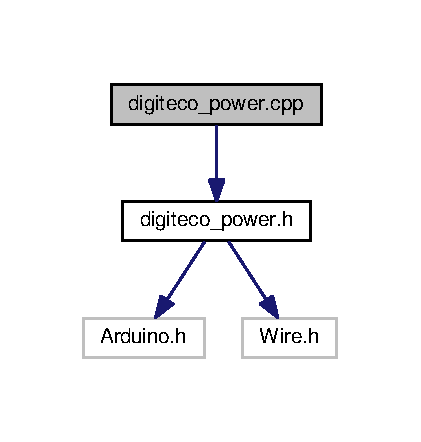
\includegraphics[width=202pt]{digiteco__power_8cpp__incl}
\end{center}
\end{figure}
\subsection*{Namespaces}
\begin{DoxyCompactItemize}
\item 
 \hyperlink{namespaceDigitecoPower}{Digiteco\+Power}
\begin{DoxyCompactList}\small\item\em \hyperlink{namespaceDigitecoPower}{Digiteco\+Power} namespace. \end{DoxyCompactList}\end{DoxyCompactItemize}
\subsection*{Functions}
\begin{DoxyCompactItemize}
\item 
bool \hyperlink{namespaceDigitecoPower_adb7461d6d597526eace685d0365732b7}{Digiteco\+Power\+::de\+\_\+read} (uint8\+\_\+t address, float $\ast$value)
\begin{DoxyCompactList}\small\item\em Read value at specified i2c-\/address. \end{DoxyCompactList}\item 
bool \hyperlink{namespaceDigitecoPower_a2a1d64ce6df863e91fef034a496220fd}{Digiteco\+Power\+::de\+\_\+send} (uint8\+\_\+t address, uint8\+\_\+t data)
\begin{DoxyCompactList}\small\item\em Send data at specified i2c-\/address. \end{DoxyCompactList}\end{DoxyCompactItemize}

\hypertarget{digiteco__power_8h}{}\section{sketchbook/libraries/\+Digiteco\+Power/digiteco\+\_\+power.h File Reference}
\label{digiteco__power_8h}\index{sketchbook/libraries/\+Digiteco\+Power/digiteco\+\_\+power.\+h@{sketchbook/libraries/\+Digiteco\+Power/digiteco\+\_\+power.\+h}}
{\ttfamily \#include $<$Arduino.\+h$>$}\newline
{\ttfamily \#include $<$Wire.\+h$>$}\newline
Include dependency graph for digiteco\+\_\+power.\+h\+:\nopagebreak
\begin{figure}[H]
\begin{center}
\leavevmode
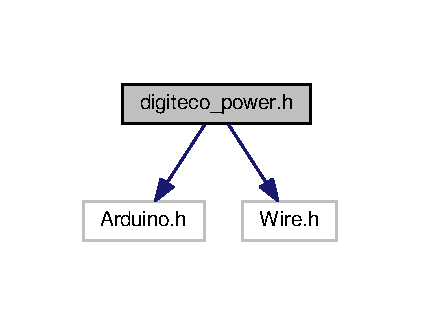
\includegraphics[width=204pt]{digiteco__power_8h__incl}
\end{center}
\end{figure}
This graph shows which files directly or indirectly include this file\+:\nopagebreak
\begin{figure}[H]
\begin{center}
\leavevmode
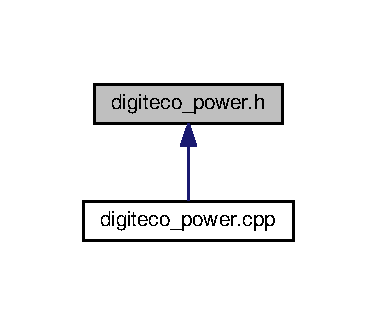
\includegraphics[width=200pt]{digiteco__power_8h__dep__incl}
\end{center}
\end{figure}
\subsection*{Namespaces}
\begin{DoxyCompactItemize}
\item 
 \hyperlink{namespaceDigitecoPower}{Digiteco\+Power}
\begin{DoxyCompactList}\small\item\em \hyperlink{namespaceDigitecoPower}{Digiteco\+Power} namespace. \end{DoxyCompactList}\end{DoxyCompactItemize}
\subsection*{Macros}
\begin{DoxyCompactItemize}
\item 
\mbox{\Hypertarget{digiteco__power_8h_aa8deb23e82d0f30f684e2cecbfc8b146}\label{digiteco__power_8h_aa8deb23e82d0f30f684e2cecbfc8b146}} 
\#define \hyperlink{digiteco__power_8h_aa8deb23e82d0f30f684e2cecbfc8b146}{D\+I\+G\+I\+T\+E\+C\+O\+\_\+\+P\+O\+W\+E\+R\+\_\+\+D\+E\+F\+A\+U\+L\+T\+\_\+\+A\+D\+D\+R\+E\+SS}~(0x30)
\begin{DoxyCompactList}\small\item\em I2C address. \end{DoxyCompactList}\item 
\mbox{\Hypertarget{digiteco__power_8h_a2f55faaba5cd777a035ef225338b7497}\label{digiteco__power_8h_a2f55faaba5cd777a035ef225338b7497}} 
\#define \hyperlink{digiteco__power_8h_a2f55faaba5cd777a035ef225338b7497}{D\+I\+G\+I\+T\+E\+C\+O\+\_\+\+P\+O\+W\+E\+R\+\_\+\+R\+E\+A\+D\+\_\+\+D\+A\+T\+A\+\_\+\+L\+E\+N\+G\+TH}~(4)
\begin{DoxyCompactList}\small\item\em Read data length in numbers of bytes. \end{DoxyCompactList}\item 
\mbox{\Hypertarget{digiteco__power_8h_a253fda21968e718264608f907bbeac5b}\label{digiteco__power_8h_a253fda21968e718264608f907bbeac5b}} 
\#define \hyperlink{digiteco__power_8h_a253fda21968e718264608f907bbeac5b}{D\+I\+G\+I\+T\+E\+C\+O\+\_\+\+P\+O\+W\+E\+R\+\_\+\+I\+N\+P\+U\+T\+\_\+\+V\+O\+L\+T\+A\+G\+E\+\_\+\+A\+D\+D\+R\+E\+SS}~(0)
\begin{DoxyCompactList}\small\item\em I2C input voltage read address. \end{DoxyCompactList}\item 
\mbox{\Hypertarget{digiteco__power_8h_ad018f5da715615cd840a6cf765d2d5bf}\label{digiteco__power_8h_ad018f5da715615cd840a6cf765d2d5bf}} 
\#define \hyperlink{digiteco__power_8h_ad018f5da715615cd840a6cf765d2d5bf}{D\+I\+G\+I\+T\+E\+C\+O\+\_\+\+P\+O\+W\+E\+R\+\_\+\+I\+N\+P\+U\+T\+\_\+\+C\+U\+R\+R\+E\+N\+T\+\_\+\+A\+D\+D\+R\+E\+SS}~(1)
\begin{DoxyCompactList}\small\item\em I2C input current read address. \end{DoxyCompactList}\item 
\mbox{\Hypertarget{digiteco__power_8h_a7094a7cbca7a206e7f9b590ef002d501}\label{digiteco__power_8h_a7094a7cbca7a206e7f9b590ef002d501}} 
\#define \hyperlink{digiteco__power_8h_a7094a7cbca7a206e7f9b590ef002d501}{D\+I\+G\+I\+T\+E\+C\+O\+\_\+\+P\+O\+W\+E\+R\+\_\+\+B\+A\+T\+T\+E\+R\+Y\+\_\+\+V\+O\+L\+T\+A\+G\+E\+\_\+\+A\+D\+D\+R\+E\+SS}~(2)
\begin{DoxyCompactList}\small\item\em I2C input battery voltage read address. \end{DoxyCompactList}\item 
\mbox{\Hypertarget{digiteco__power_8h_a1c83becacdace25fd429d805f9db0cc6}\label{digiteco__power_8h_a1c83becacdace25fd429d805f9db0cc6}} 
\#define \hyperlink{digiteco__power_8h_a1c83becacdace25fd429d805f9db0cc6}{D\+I\+G\+I\+T\+E\+C\+O\+\_\+\+P\+O\+W\+E\+R\+\_\+\+B\+A\+T\+T\+E\+R\+Y\+\_\+\+C\+U\+R\+R\+E\+N\+T\+\_\+\+A\+D\+D\+R\+E\+SS}~(3)
\begin{DoxyCompactList}\small\item\em I2C input battery current read address. \end{DoxyCompactList}\item 
\mbox{\Hypertarget{digiteco__power_8h_a094fe61fa8191acc80dde2d138df28c7}\label{digiteco__power_8h_a094fe61fa8191acc80dde2d138df28c7}} 
\#define \hyperlink{digiteco__power_8h_a094fe61fa8191acc80dde2d138df28c7}{D\+I\+G\+I\+T\+E\+C\+O\+\_\+\+P\+O\+W\+E\+R\+\_\+\+B\+A\+T\+T\+E\+R\+Y\+\_\+\+C\+H\+A\+R\+G\+E\+\_\+\+A\+D\+D\+R\+E\+SS}~(4)
\begin{DoxyCompactList}\small\item\em I2C input battery charge percentage read address. \end{DoxyCompactList}\item 
\mbox{\Hypertarget{digiteco__power_8h_a5a99a63cee1474307f90a3ab572c4eb3}\label{digiteco__power_8h_a5a99a63cee1474307f90a3ab572c4eb3}} 
\#define \hyperlink{digiteco__power_8h_a5a99a63cee1474307f90a3ab572c4eb3}{D\+I\+G\+I\+T\+E\+C\+O\+\_\+\+P\+O\+W\+E\+R\+\_\+\+O\+U\+T\+P\+U\+T\+\_\+\+V\+O\+L\+T\+A\+G\+E\+\_\+\+A\+D\+D\+R\+E\+SS}~(5)
\begin{DoxyCompactList}\small\item\em I2C output voltage read address. \end{DoxyCompactList}\end{DoxyCompactItemize}
\subsection*{Functions}
\begin{DoxyCompactItemize}
\item 
bool \hyperlink{namespaceDigitecoPower_adb7461d6d597526eace685d0365732b7}{Digiteco\+Power\+::de\+\_\+read} (uint8\+\_\+t address, float $\ast$value)
\begin{DoxyCompactList}\small\item\em Read value at specified i2c-\/address. \end{DoxyCompactList}\item 
bool \hyperlink{namespaceDigitecoPower_a2a1d64ce6df863e91fef034a496220fd}{Digiteco\+Power\+::de\+\_\+send} (uint8\+\_\+t address, uint8\+\_\+t data)
\begin{DoxyCompactList}\small\item\em Send data at specified i2c-\/address. \end{DoxyCompactList}\end{DoxyCompactItemize}

%--- End generated contents ---

% Index
\backmatter
\newpage
\phantomsection
\clearemptydoublepage
\addcontentsline{toc}{chapter}{Index}
\printindex

\end{document}
